%!TEX root=../document.tex

\section{Ergebnisse}

\subsection{Zwei eigene Klassen (Consumer und Producer) erben von Thread (E1 und V1)}

\begin{lstlisting}[language=python]
import threading
class E1(threading.Thread):
class V1(threading.Thread):
\end{lstlisting}

\subsection{Die zwei Klassen sind über einen Queue verbunden}

Derselbe Konstruktor in beiden Klassen:\\
\begin{lstlisting}[language=python]
    def __init__(self, queue):
        """

        :param queue: Die queue welche auch der verbraucher thread hat
        """
        threading.Thread.__init__(self)
        self.queue = queue
\end{lstlisting}

\subsection{E1 sucht nach Primzahlen, ueber Queue an V1}

\begin{lstlisting}[language=python]
       def run(self):
        number = 2  #eine lokale variable, beginnt ab 2 da 0,1,2 keine Primzahlen sind
        b = True
        while number < 10000:#bIS 10000 sucht das Programm nach Primzahlen
            number += 1 #+1 zaehler
            b = True    #lokale variable zum pruefen ob die zahl eine prmzahl ist
            for i in range(2, number):  #for schleife zum pruefen ob primzahl
                if number % i == 0:
                    b = False   #falls keine primzahl(ohne rest dividierbar)
                    break
            if b == True:   #falls es doch eine primzahl ist bleibt b true und somit wird
                            #hier dann auch queue.put benuzt um den verbraucher zu
                            # benachrichtigen
                self.queue.put(number)
                self.queue.join()
        number = "fertig"   #den verbraucher benachrichtigen das die zaehlung vorbai ist
        self.queue.put(number)  #den verbraucher benachrichtigen das die zaehlung
                                # vorbai ist

\end{lstlisting}

\subsection{V1 gibt empfangene Zahl aus und schreibt in ein text file}

\begin{lstlisting}[language=python]
  def run(self):
        tf = open("output.txt", "w")    #oeffnen des text files, "w" ->
                                        # falls keins vorhanden -> neu erstellen
                                        #falsl doch -> ueberschreiben
        while True:
            number = self.queue.get()   #erhaellt die variable aus der queue und
                                        # signalisiert das der erzeuger weitermachen kann
            if(number == "fertig"):     #prueft ob die zaehlung vorbei ist
                break
            print("Primzahl: %d" % number)  #ausgabe in die konsole
            self.queue.task_done()
            tf.write("Primzahl: " + str(number) + "\n") #schreiben in das text file
\end{lstlisting}
\clearpage
\subsection{Der ganze Code}

\begin{lstlisting}[language=python]
import threading
import queue

class E1(threading.Thread):
    def __init__(self, queue):
        """

        :param queue: Die queue welche auch der verbraucher thread hat
        """
        threading.Thread.__init__(self)
        self.queue = queue

    def run(self):
        number = 2  #eine lokale variable, beginnt ab 2 da 0,1,2 keine Primzahlen sind
        b = True
        while number < 10000:#bIS 10000 sucht das Programm nach Primzahlen
            number += 1 #+1 zaehler
            b = True    #lokale variable zum pruefen ob die zahl eine prmzahl ist
            for i in range(2, number):  #for schleife zum pruefen ob primzahl
                if number % i == 0:
                    b = False   #falls keine primzahl(ohne rest dividierbar)
                    break
            if b == True:   #falls es doch eine primzahl ist bleibt b true und somit wird
                            #hier dann auch queue.put benuzt um den verbraucher zu
                            # benachrichtigen
                self.queue.put(number)
                self.queue.join()
        number = "fertig"   #den verbraucher benachrichtigen das die zaehlung vorbai ist
        self.queue.put(number)  #den verbraucher benachrichtigen das die zaehlung
                                # vorbai ist

class V1(threading.Thread):
    def __init__(self, queue):
        """

        :param queue: Die queue welche auch der verbraucher thread hat
        """
        threading.Thread.__init__(self)
        self.queue = queue

    def run(self):
        tf = open("output.txt", "w")    #oeffnen des text files, "w" ->
                                        # falls keins vorhanden -> neu erstellen
                                        #falsl doch -> ueberschreiben
        while True:
            number = self.queue.get()   #erhaellt die variable aus der queue und
                                        # signalisiert das der erzeuger weitermachen kann
            if(number == "fertig"):     #prueft ob die zaehlung vorbei ist
                break
            print("Primzahl: %d" % number)  #ausgabe in die konsole
            self.queue.task_done()
            tf.write("Primzahl: " + str(number) + "\n") #schreiben in das text file

if __name__ == "__main__":
    queue = queue.Queue()
    t1 = E1(queue)
    t2 = V1(queue)
    t1.start()
    t2.start()
    t1.join()
    t2.join()
\end{lstlisting}
\clearpage
\subsection{Consol Outpu bei Eingabe 1000}
\begin{figure}[!h]
	\begin{center}
		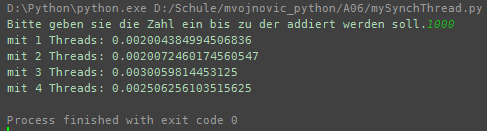
\includegraphics[width=0.7\linewidth]{images/consolOutput.png}
		\caption{Consolen Output}
		\label{broker}
	\end{center}
\end{figure}